\documentclass{standalone}
\usepackage[x11names]{xcolor}
\usepackage{tikz}
\usetikzlibrary{decorations.pathmorphing}
\usetikzlibrary{decorations.pathreplacing}
\tikzset{sdot/.style = {fill, circle, inner sep = 1.5pt}}


\begin{document}

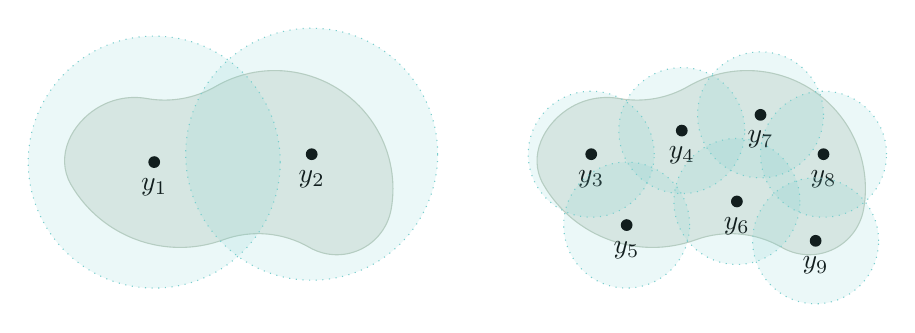
\begin{tikzpicture}
    \filldraw [Honeydew3, fill opacity = 0.4] (0, 0) arc (120:80:0.9) arc (260:300:1.3) arc (120:-10:1.5) arc (350:240:0.7) arc (60:110:1.3) arc (290:210:1.6) to [out = 120, in = 210] (0, 0);
    \foreach \x\y\i in {0.7/-0.7/1, 2.7/-0.6/2} {
        \node [label = below: {$y_\i$}] (y\i) [sdot] at (\x, \y) {};
        \filldraw [DarkSlateGray3, fill opacity = 0.15, dotted] (y\i) circle (1.6);
    }
    \begin{scope}[xshift = 6cm]
        \filldraw [Honeydew3, fill opacity = 0.4] (0, 0) arc (120:80:0.9) arc (260:300:1.3) arc (120:-10:1.5) arc (350:240:0.7) arc (60:110:1.3) arc (290:210:1.6) to [out = 120, in = 210] (0, 0);
        \foreach \x\y\i in {0.25/-0.6/3, 1.4/-0.3/4, 0.7/-1.5/5, 2.1/-1.2/6, 2.4/-0.1/7, 3.2/-0.6/8, 3.1/-1.7/9} {
            \node [label = below: {$y_\i$}] (y\i) [sdot] at (\x, \y) {};
            \filldraw [DarkSlateGray3, fill opacity = 0.15, dotted] (y\i) circle (0.8);
        }
    \end{scope}
\end{tikzpicture}
\end{document}